% Secondary material moved from the preceding paper. The previous publication remains in Git history.
\section{Historical local-model studies and supplementary derivations}
\label{sec:paper-history}
This supplement preserves the local-model experiments, reverse-construction details, restricted exact examples, and derivations removed from the main paper. Their controls and physical domains remain separate from the new shared-model comparison. The following subsections retain the earlier experimental statements and their original scope.
\subsection{Feynman integrals and their reduction with Kira}
\label{history:sec:reduction}
\subsubsection{Families, indices, and sectors}
An integral family specifies a set of propagators and the external scalar products. Integrals in the same family differ in the integer powers assigned to those propagators~\cite{Weinzierl2022,KiraOriginal}:
\begin{equation}
 I_{\boldsymbol a}(\boldsymbol x,d)
 =\int\prod_{h=1}^{L}\frac{d^d\ell_h}{i\pi^{d/2}}
       \prod_{i=1}^{N}D_i^{-a_i},
 \qquad D_i=q_i^2-m_i^2+i0.
 \label{history:eq:family}
\end{equation}
Here $L$ is the number of loops, $\ell_h$ is the momentum of loop $h$, and $N$ is the number of inverse propagators, including any auxiliary entries. The momentum $q_i$ is a linear combination of loop and external momenta, and $m_i$ is the corresponding mass. The term $i0$ specifies the Feynman prescription. We use dimensional regularization with $d=4-2\epsilon$, where $\epsilon$ is the regulator, and collect the independent momentum invariants and squared masses in $\boldsymbol x$.

The index $a_i$ determines how $D_i$ enters the integrand. A positive index places it in the denominator, a zero index removes it, and a negative index places a power of it in the numerator. Auxiliary inverse propagators represent scalar products that cannot be expressed using the physical propagators alone. Integrals with the same set of positive indices belong to the same \emph{sector}~\cite{KiraOriginal}. A top sector specifies a maximal declared set of positive propagator indices, and its subsectors follow by removing propagators~\cite{KiraOriginal}. These definitions give Kira a common way to label the integrals and organize the equations between them.

\subsubsection{From an IBP identity to a master-integral reduction}
An IBP identity starts from an index vector $\boldsymbol\sigma$, called a \emph{seed}. We multiply its integrand by a loop or external momentum $v$, differentiate with respect to a loop momentum $\ell_k$, and integrate the total derivative. Dimensional regularization gives~\cite{ChetyrkinTkachov}
\begin{equation}
 0=\int\prod_h\frac{d^d\ell_h}{i\pi^{d/2}}
 \frac{\partial}{\partial\ell_k^\mu}
 \left(v^\mu\prod_iD_i^{-\sigma_i}\right)
 =\sum_j A_{\boldsymbol\sigma,o;j}(\boldsymbol x,d)
     I_{\boldsymbol a^{(j)}}.
 \label{history:eq:ibp}
\end{equation}
The label $o$ specifies the derivative through the choices of $k$ and $v$, while $j$ labels the integrals produced when the derivative is expanded. The coefficient $A_{\boldsymbol\sigma,o;j}$ multiplies integral $I_{\boldsymbol a^{(j)}}$ in that identity. Since several operators can act on the same seed, one seed generally generates several equations. Appendix~\ref{history:app:ibp} derives the shifts in the integral indices and the row operation used to eliminate an integral.

Kira generates these equations within prescribed index limits, applies symmetry relations, removes redundant equations, and solves the remaining system~\cite{KiraOriginal,Kira3}. Each equation forms a row of the coefficient matrix, and each integral corresponds to a column. Elimination combines rows to remove integrals in the chosen order; back-substitution then expresses the requested targets in terms of the remaining masters. Kira can manipulate symbolic rational functions directly or use exact arithmetic modulo a prime, with reconstruction when a symbolic result is required~\cite{KiraOriginal,Kira2}. Arithmetic modulo a prime takes place in a finite field, so its numerical appearance does not introduce floating-point error.

A requested target may be a single indexed integral or a linear combination $T=\sum_u c_u I_{\boldsymbol a^{(u)}}$. The desired result is
\begin{equation}
 T=\sum_{m=1}^{n_M}r_{Tm}(\boldsymbol x,d)M_m,
 \qquad r_{Tm}\in\Q(\boldsymbol x,d).
 \label{history:eq:master}
\end{equation}
Here $c_u$ is the coefficient of a target term, $M_m$ is master integral $m$, and $n_M$ is the number of masters. The field $\Q(\boldsymbol x,d)$ consists of rational functions of the invariants, squared masses, and dimension with rational-number coefficients. Reduction determines the coefficients $r_{Tm}$; evaluating the master integrals is a separate part of the amplitude calculation.

\subsubsection{Where learned choices can reduce the work}
Table~\ref{history:tab:decisions} identifies the three decisions studied here. Seed selection changes which groups of identities are available, row selection changes the elimination steps, and equation selection can suppress an individual seed--operator pair before Kira constructs its coefficients. We use \emph{native choices} to mean Kira's own decision rules. A learned model changes a decision, while Kira continues to carry out the exact algebra.

Every completed target must reach the prescribed master basis. In the comparisons, we also check its coefficients against an independently obtained exact reduction. If a chosen seed set or equation set is insufficient, the calculation repeats with native choices or a larger seed region. We call this repeated attempt a \emph{fallback} and include its cost in the reported time. Thus the relevant question for each model is whether the work it avoids exceeds the cost of prediction and any fallback.

\begin{table}[!htbp]
\centering\small
\caption{The three decisions and the work each model can avoid.}
\label{history:tab:decisions}
\begin{tabularx}{\linewidth}{@{}lYY@{}}\toprule
Model & Decision & Possible saving\\\midrule
Seed and batch selection & Which seed regions and target groups should Kira use? & Limit equation generation and repeated work.\\
Row selection & Which allowed row eliminates the next integral? & Reduce intermediate expressions and operations.\\
Equation selection & Which seed--operator pairs are useful? & Avoid constructing unnecessary coefficients.\\\bottomrule
\end{tabularx}
\end{table}

The following comparisons retain native row elimination. The original row network took 1.305 times the stock reduction time in 84 exact trials, while a later compiled row policy gave a ratio of $0.982$ with interval $[0.959,1.003]$. We therefore omit learned row choice and focus on seed regions and equations. Appendix~\ref{history:sec:rows} gives the models and checks behind that decision.

\subsection{Overall performance and physical scope}
% BEGIN FAMILY COST OVERALL
The final combined comparison in Section~\ref{sec:family-cost} gives time ratio 0.855 against the preceding native control, 0.961 against the previous application, and isolated learned-to-fixed ratio 0.991 with validation-selected exact routes in both controls. These ratios use 41 matched batches, five repetitions, and complete process times. The following paragraphs retain the earlier comparisons and their separate physical domains.
% END FAMILY COST OVERALL

\label{history:sec:overall}
% BEGIN BANANA OVERALL
The separate analytic specialization reduces scalar massless banana targets through one corner master, with a derived coefficient valid at every positive loop count. Its 9 completed native comparisons give a speedup of 21.3--357.8 times for the stated targets. These gains come from exact mathematics and are separate from the ML gains (Section~\ref{sec:banana}).
% END BANANA OVERALL
\subsubsection{What the model comparisons establish}
% BEGIN JOINT POLICY OVERALL
Section~\ref{sec:joint-policy} retains the preceding ML application because neither new joint predictor clears the 2\% validation threshold. On 24 first requests, the retained application with the new interface gives 1.2\% less time, with time-ratio interval $[0.975,1.024]$ relative to its preceding interface. This difference supplies no evidence of a gain from the new predictors. The separate scale sequences give 64.4\% less time than the preceding application without reuse, including the initial Kira solve. This additional saving comes from the derived scale identity, while the first reduction still uses the preceding ML decisions.
% END JOINT POLICY OVERALL

% BEGIN SEED GEOMETRY OVERALL
The first evolved seed boundary gives 22.3\% less time, with a paired-repetition ratio interval of $[0.751, 0.813]$ relative to tuned native Kira on eight planar two-loop requests. Its added saving relative to the fixed surrounding-width control is 6.5\% less time, with a paired-repetition ratio interval of $[0.899, 0.980]$. The broader sparse-seed workflow in Section~\ref{sec:seed-geometry} gives 22.2\% less time, with a paired-repetition ratio interval of $[0.764, 0.792]$ relative to tuned native Kira on 20 matched two-loop requests. Its comparison with the fixed sparse control gives 3.6\% less time, with a paired-repetition ratio interval of $[0.946, 0.981]$. These results use separate workloads from the earlier equation-filter and batch tests.
% END SEED GEOMETRY OVERALL

% BEGIN BATCH POLICY OVERALL
The target-batch comparison in Section~\ref{sec:batch-policy} gives 1.5\% more time than the previous undivided workflow across 96 matched batches with up to 11 targets. Its additional change relative to fixed partitions with the same filters is 0.8\% more time, with ratio interval $[0.988, 1.035]$. Validation disables the new predictor, so this comparison establishes no additional ML gain from batch selection. Every successful reduction passes exact coefficient checks. This is a separate workload from the smaller-batch filter study.
% END BATCH POLICY OVERALL
% BEGIN EQUATION REFINEMENT OVERALL
After fixed seed tuning, newly trained equation filters give 8.0\% less complete time on 32 matched batches where validation enables them, with 4.8\% time saving across all 68 matched batches. These controls disable all ML and retain the same seed settings and exact implementation. Section~\ref{sec:equation-refinement} gives the failures, timing intervals, and physical limits.
% END EQUATION REFINEMENT OVERALL

% BEGIN LEARNED BOUNDS SUMMARY
The new seed-bound study in Section~\ref{sec:learned-bounds} isolates a learned choice with all earlier models disabled. On 68 matched nontrivial batches, complete application time changes from 164.926 seconds under native bounds and 119.717 seconds under tuned fixed settings to 119.081 seconds with the new model. This gives 27.8\% less time than native bounds and 0.5\% less time than the tuned fixed control. The comparison includes model loading, native IBP generation, exact reduction, coefficient checks, and recovery, with a supplied basis. It uses known structures at one through four loops and separate rational profiles; the additional saving over tuned fixed settings remains within timing variation.
% END LEARNED BOUNDS SUMMARY
The broader coverage study in Section~\ref{sec:coverage} defines 90 native-family requests through twelve loops. The current interface accepts 54 of them, and 39 complete three checked nontrivial full reductions with revised preparation. On 37 matched completed requests, the revised full calculation takes 88.2\% less time than the saved original Kira executable. The supplied-basis selected application takes 0.1\% less time than the revised native control on its separate matched set. The approximately 0.1\% difference from the revised native control establishes no reliable additional learned gain on this wider set. Unsupported, failed, and identity-only requests remain outside these timing ratios.

The preparation comparison keeps every trained model fixed and reduces exact preparation around its decisions. On 26 new batches, complete time changes from 79.784 to 64.183 seconds, or 19.6\% less time. Section~\ref{sec:parametric} gives the matched controls and graph results. With the revised preparation held fixed, the selected portfolio uses 4.7\% less time than the fixed portfolio by summed medians and 5.0\% less time across all repetitions. The previous portfolio study in Section~\ref{sec:portfolio} remains a separate comparison on different targets.

The earlier model tests and the exact preprocessing study answer separate questions. Seed and equation selection help in their measured domains, while learned row selection remains omitted. Exact preprocessing reduces costs shared by every portfolio candidate. Restricted vacuum recurrence and repeated-request reuse supply further savings under their own assumptions. These experiments use different inputs and controls, so their speedup factors cannot be multiplied.

\begin{table}[!htbp]
\centering\small
\caption{Summary of separate comparisons. Each row uses its stated inputs and baseline. The studies provide no measured product of these speedups.}
\label{history:tab:overall}
\begin{tabularx}{\linewidth}{@{}lYY@{}}\toprule
Method & Tested calculation & Result for complete time\\\midrule
% BEGIN SEED GEOMETRY TABLE
Evolved seed boundary & Eight planar two-loop targets & 22.3\% less time than tuned native; 6.5\% less time than fixed width\\
Sparse-seed deployment & 20 planar and nonplanar targets & 22.2\% less time than tuned native; 22.6\% less time than previous\\
% END SEED GEOMETRY TABLE
% BEGIN JOINT POLICY TABLE
Retained ML, new interface & 24 first requests; two-loop boxes & 1.2\% less time than previous; 5.7\% less time than fixed\\
Scale reuse with ML & Four three-scale sequences & 64.4\% less time than previous, including first solve\\
% END JOINT POLICY TABLE

% BEGIN BATCH POLICY TABLE
Target batch choice & 96 matched batches; up to 11 targets & 1.5\% more time than previous; 0.8\% more time than fixed partitions\\
% END BATCH POLICY TABLE
% BEGIN EQUATION REFINEMENT TABLE
Trained equation filters & 68 matched batches; loops 1--4 & 4.8\% less time than tuned ML-off control; 8.0\% on 32 active batches\\
% END EQUATION REFINEMENT TABLE
% BEGIN LEARNED BOUNDS TABLE
Learned seed bounds & 68 matched batches; loops 1--4 & 27.8\% less time than native bounds; 0.5\% less than tuned fixed settings\\
% END LEARNED BOUNDS TABLE
% BEGIN FINAL PORTFOLIO SUMMARY
Revised exact preparation & Fresh known-graph batches, loops 1--4 & 19.6\% less time than the previous implementation\\
Added outer prediction & Same revised preparation & 4.7\% less time by medians; 5.0\% less across repetitions\\
% END FINAL PORTFOLIO SUMMARY
% BEGIN CURRENT COST SUMMARY
Earlier cost model & Known graph structures, loops 1--4 & 0.5\% less time than native choices in the improved executable\\
Earlier gated policy & Same targets; fixed settings selected per graph & 1.8\% less time than the graph-specific fixed control\\
% END CURRENT COST SUMMARY
Seed network & One target from an existing equation pool & 8.6\% less time\\
Equation tree & Native reduction in four trained graph structures & 5.7\% less time\\
Row policy & Native symbolic elimination & No reliable saving\\
Original equation tree & Three new scattering structures & 25.2\% more time\\
Complete-cost model & Seven known graph structures, loops 1--3 & No reliable gain over native controls\\
Policies per graph & Higher powers and lower sectors, loops 1--3 & 6.3\% less time\\
Selective seed expansion & Known graphs, new profiles, loops 1--3 & 14.8\% less time than native\\
Selecting Kira workers & Known graphs, new profiles, loops 1--3 & 4.2\% less time than previous, sum of medians\\
Choosing Kira settings & Known graphs, new profiles, loops 1--3 & No added gain over preceding method\\
Joint integrated reduction & Two compatible requests in seven graph structures & 48.3\% less time\\
Exact recurrences and reuse & Restricted vacuum family, loops 1--12 & $543.8\times$ faster\\\bottomrule
\end{tabularx}
\end{table}

\subsubsection{Exact reuse in the restricted vacuum family}
The high-loop vacuum study explores a different source of acceleration. For the family in Appendix~\ref{history:app:vacuum}, exact recurrences express the reduction coefficients through $z=L(d-2)$. A coefficient calculation can then serve several loop orders and several targets. The method reuses intermediate coefficients and checks each result with an independent Taylor expansion; Kira remains available if this direct check fails. The deployed recurrence uses a fixed rule. Its large saving comes from exact mathematical reuse and implementation changes. A separately trained selector for recurrence strategies takes 1.7\% more time than the fixed rule and supplies no established additional saving.

The comparison uses eight fresh groups, each containing three mass profiles with two, three, or four massive denominators, and requests loop orders one through twelve. Five repetitions compare the saved original Kira 3.1 executable, a later full-pool control, and the recurrence method on identical requests. All 120 calculations pass exact checks. The final-to-original time ratio is $0.001839$, corresponding to speedup $543.815$ with interval $[488.134,605.064]$. A separate check verifies 27,960 nonzero target--master coefficient polynomials. The successful recurrence calculations need no Kira calls, whereas each baseline makes 1,440 calls across its trials.

\begin{figure}[tbp]
\centering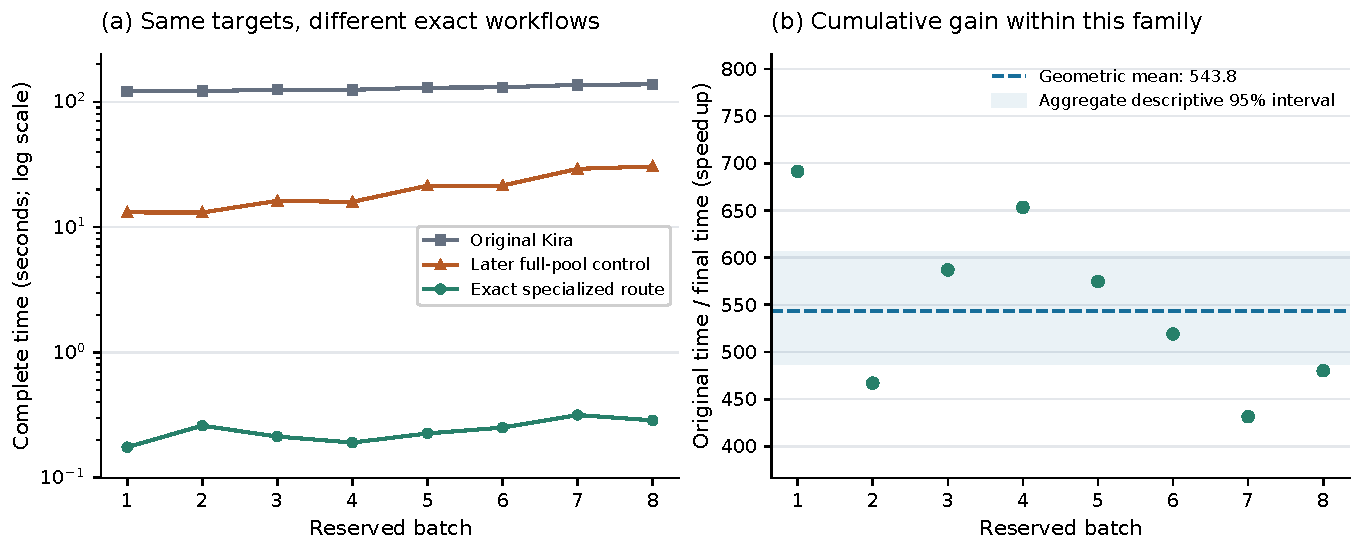
\includegraphics[width=\linewidth]{paper_figures/cumulative_results.pdf}
\caption{Exact recurrence reuse gives the large saving in the restricted vacuum family. Left: complete times on a logarithmic axis. Right: original time divided by final time. Each batch contains three mass profiles at loops 1--12. The result combines mathematical reuse and program improvements.}
\label{history:fig:cumulative}
\end{figure}

This result depends on the structure of the family. The benchmark constructs Euler and mass partial-fraction identities rather than a general high-loop IBP system. Earlier checks at loop orders 13, 16, 24, and 32 use the same family, and the recurrence proof applies to every positive integer loop order under its stated assumptions. The demonstrated high-loop result therefore concerns this restricted vacuum problem; the connected scattering comparisons in Sections~\ref{sec:components} and~\ref{sec:adaptive} have separate definitions and timings.

\subsection{Training data and experimental design}
\label{history:sec:data}
\subsubsection{Constructing targets with known reductions}
To train the original models, we need targets together with master coefficients and a recorded sequence of valid reduction steps. We obtain these data by working backwards from checked master relations. If $E_q=\sum_i A_{qi}I_i=0$ is a source identity, we construct
\begin{equation}
 T=\sum_m r_mM_m+\sum_q\lambda_qE_q,
 \qquad \lambda_q,r_m\in\Q(\boldsymbol x,d).
 \label{history:eq:reverse}
\end{equation}
Expanding the right-hand side produces an expression in indexed integrals while the added zero identities leave its master coefficients unchanged. We record the identities, their seeds and operators, and the operations used in the construction. Appendix~\ref{history:app:construction} proves the relation and explains how to recover a reduction path from this record.

This procedure usually produces a sum of integrals. It produces a single indexed integral only when the expanded expression has that form. It also supplies one sufficient seed set and one valid reduction path; it does not establish that either has minimum cost. The labels therefore teach the original models to reproduce a checked construction, and later timing experiments determine whether their choices help Kira.

\subsubsection{Coverage and separation of training and test data}
Table~\ref{history:tab:data} summarizes the original collection. The 17,100 family instances contain 57,979 master entries, counted separately in each family, and 2,301,272 targets. Many instances are parameter variations of the same graph. We call a specified assignment of masses and momentum invariants a \emph{parameter profile}. In particular, the higher-loop additions use the restricted vacuum family derived in Appendix~\ref{history:app:vacuum}; they do not represent general scattering graphs through twelve loops. The test set contains 148,494 single integrals and 541,888 integral expressions. Appendices~\ref{history:app:families} and \ref{history:app:basis} specify the families and the checks used to establish their master bases.

\begin{table}[!htbp]
\centering\small
\caption{Original constructed data. Family instances include parameter variations of the same graph.}
\label{history:tab:data}
\begin{tabular}{@{}lrr@{}}\toprule
Part & Family instances & Targets\\\midrule
Training & 11,963 & 1,610,890\\
Testing & 5,137 & 690,382\\
Total & 17,100 & 2,301,272\\\bottomrule
\end{tabular}
\end{table}

Related mass assignments remain in the same training or test group at every loop order. The seed and row networks each receive twenty additional passes through the expanded training set, starting from their earlier parameters and optimizer state. Some test profiles had already appeared in earlier evaluations, so these results concern reserved parameter groups rather than entirely new graph structures. The later native-Kira studies use separate training, validation, and test samples: training fits the models, validation selects their settings, and the reserved test measures those fixed choices.

\subsubsection{What the timing comparisons measure}
Within each comparison, every method receives the same targets and prescribed master basis and uses the same allocated resources. We use \emph{complete reduction time} for the measured time that includes input preparation, model prediction, algebra, checks, and all fallback attempts. Offline training and the construction of reference answers are excluded. The original local-model comparisons repeat each calculation five times. The final complete-cost comparisons use three repetitions, with the method order rotated. Each comparison reports batch medians and states its repetition count.

The baseline also needs to be specified. Most native comparisons use the same modified Kira 3.1 executable for learned and native choices, so improvements shared by that executable do not count as a benefit of the model. The cumulative vacuum comparison instead uses the saved original executable as its baseline. Later sections also distinguish the sum of batch median times from a geometric mean that gives each graph equal weight. The latter averages logarithms of time ratios and then exponentiates the result. Appendix~\ref{history:app:timing} defines these measures and their descriptive uncertainty intervals. Keeping these conditions explicit allows each speedup to be interpreted against the calculation it actually measures.

\subsection{Learning the three reduction decisions}
\label{history:sec:local-models}
We first test the three decisions separately. For each model, we describe the information it receives, the reference labels used in training, and its effect on exact reduction time. This separates the ability to reproduce a recorded choice from the ability to accelerate Kira.

\subsubsection{Model 1: selecting seeds}
\label{history:sec:seeds}
The seed network receives the terms of the target, its family, the master indices, and a finite list of candidate seeds. It maps each target term to 32 learned numerical features and combines these with ordered pairs of terms and information about the family and masters. A seed-dependent attention operation then identifies which target terms are most relevant to that candidate. The shared representations and attention follow Refs.~\cite{DeepSets,AttentionIsAllYouNeed}; Appendix~\ref{history:app:models} gives the full architecture.

The network has 28,097 fitted parameters and assigns a separate score to every candidate:
\begin{equation}
 p_b=\frac{1}{1+e^{-g_\theta(T,F,\mathcal M,\boldsymbol\sigma_b)}},
 \qquad
 \widehat\Sset(T)=\{\boldsymbol\sigma_b\in\Cset:p_b\geq\tfrac12\}.
 \label{history:eq:seed}
\end{equation}
Here $F$ denotes the family, $\mathcal M$ the master list, $\Cset$ the candidate list, and $g_\theta$ the output of the network with fitted parameters $\theta$. The score estimates whether a seed belongs to the recorded sufficient set. Because a target can require several seeds, several scores can exceed the selection threshold and their sum need not be one. Training uses binary cross-entropy and AdamW~\cite{AdamW}. The network receives neither the target's final master coefficients nor its later reduction steps.

On the 690,382 reserved targets, the model has precision 95.750\%, recall 96.892\%, and $F_1$ score 96.318\%. Its complete predicted set matches the recorded set for 84.332\% of targets. Kira reduces 652,517 targets with the predicted sets, corresponding to 94.515\% sufficiency, and reduces all targets when the full equation pool is available. These percentages differ because matching the recorded set and supplying enough equations are different tests: another seed set can also be sufficient. Appendix~\ref{history:app:timing} defines the metrics. We report precision and recall because the large number of negative labels can make overall classification accuracy misleading~\cite{SaitoRehmsmeier2015}.

To determine whether this prediction saves time, we use a separate comparison on existing identity pools from twelve reserved one-loop box instances. The weights remain fixed, and the timing test uses threshold $0.01$, chosen before that comparison; the earlier label and sufficiency tests use $1/2$. Both the learned selector and a distance-based rule receive the same basis check and full-pool fallback. For single targets, the learned-to-full-pool time ratio is $0.914$, with descriptive 95\% interval $[0.871,0.958]$, giving 8.6\% less time. Relative to the distance rule, the ratio is $0.913$ with interval $[0.855,0.972]$, giving 8.7\% less time. Every method completes all five repetitions of these twelve cases.

The gain is less clear for larger requests. For sixteen-target batches, the ratio is $0.952$ with interval $[0.772,1.148]$, which includes equal time. Across the full planned seed comparison, 345 trials finish exactly, three remain incomplete, and twelve repetitions are skipped; the timing summary uses only complete paired cases. The identity pools already exist when these timers start. A separate native test that includes IBP generation gives ratio $1.096$ with interval $[0.963,1.275]$. Thus the original network demonstrates a saving for the stated supplied-equation single-target test, while native generation requires a different assessment. Section~\ref{history:sec:adaptation} reports new seed trees trained directly on scattering reductions.

\begin{figure}[tbp]
\centering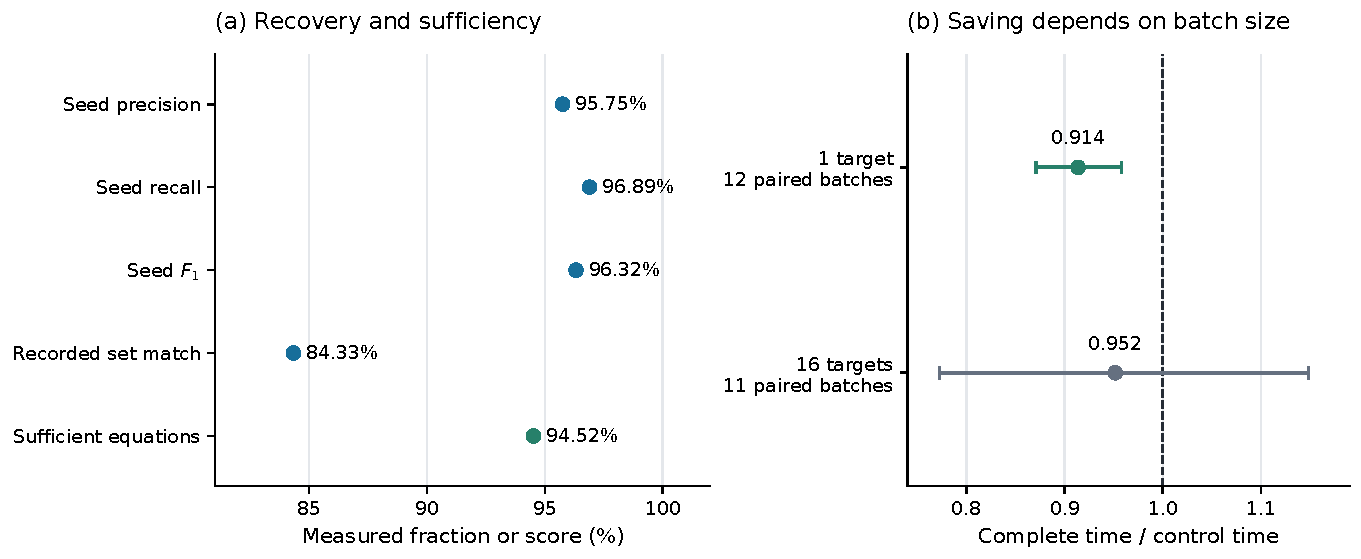
\includegraphics[width=\linewidth]{paper_figures/seed_results.pdf}
\caption{Seed prediction accuracy and reduction speed measure different outcomes. Left: results on the original reserved targets. Right: learned time divided by full-pool time. Values below one are faster. The single-target interval lies below one; the sixteen-target interval crosses it.}
\label{history:fig:seed}
\end{figure}

\FloatBarrier

\subsubsection{Model 2: selecting elimination rows}
\label{history:sec:rows}
After the equations have been generated, several allowed source rows may eliminate the next integral. The row network scores these alternatives using 132 inputs that describe the pivot integral, nonzero entries, family, matrix size, and sampled cancellations. It maps each action to 32 learned features, combines information across the available actions, and passes the result through a hidden layer with 64 components. A softmax converts the final scores into probabilities that sum to one, and the network selects the action with the largest probability. The 10,529 fitted parameters determine the choice; exact arithmetic performs the row operation. Appendices~\ref{history:app:ibp} and \ref{history:app:models} give the operation and architecture.

The original training examples follow one changing target row while the source identities stay fixed. On 2,558,472 reserved states with a choice, the network selects the recorded action in 95.845\% of cases, compared with 99.473\% for a local deterministic rule. Complete predicted paths agree with the saved master row at three finite-field points for 690,302 of 690,382 targets. These sampled checks support agreement at those points but do not prove symbolic equality. Including prediction, the network takes 17.657 times as long as the local rule.

The more relevant application places the fixed network inside Kira's changing symbolic matrix and preserves Kira's allowed integral order. Across 84 exactly checked trials, this implementation takes 1.305 times the time of stock Kira. We therefore also test smaller policies trained on measured algebraic cost, with compiled prediction and shared features. The latest row-only comparison gives ratio $0.982$ with interval $[0.959,1.003]$, while combining it with the seed policy gives $1.100$ with interval $[0.966,1.279]$ against native choices.

Figure~\ref{history:fig:row} shows that the later intervals still include equal time. We therefore retain Kira's row choices in the final method. This result explains why the remaining studies focus on decisions that can avoid equation generation or repeated work: reproducing a plausible elimination path did not, by itself, provide a reliable reduction in complete time.

\begin{figure}[tbp]
\centering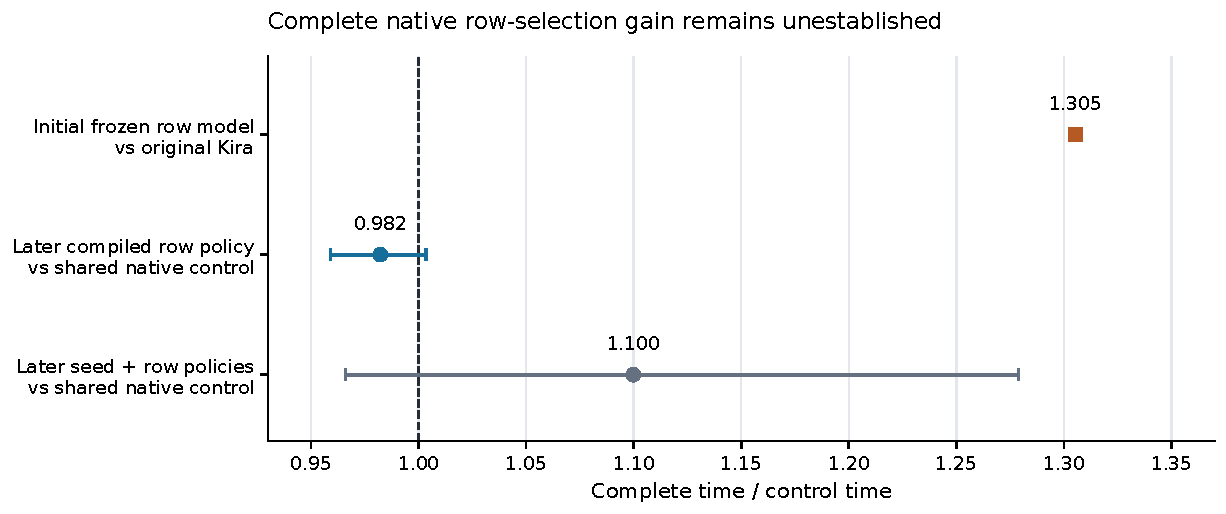
\includegraphics[width=0.96\linewidth]{paper_figures/row_results.pdf}
\caption{The row model gives no reliable complete-time saving. The first model is slower, and the later row-only interval includes equal time. The original summary provides no interval for the first result. These comparisons use different model versions.}
\label{history:fig:row}
\end{figure}

\FloatBarrier

\subsubsection{Model 3: selecting individual equations}
\label{history:sec:equations}
Equation selection offers an earlier opportunity to avoid work. The model scores each seed--operator pair before Kira constructs its symbolic coefficients. Its seventeen inputs describe the family, target list, seed indices, and operator; they include the number of loops and targets, extra propagator powers, numerator rank, and distance between seed and target indices. A classification tree~\cite{CART1984} applies feature-threshold decisions and returns a score from its final leaf. The score estimates whether the equation belongs to the useful part of a recorded native reduction. No equation coefficients are needed for prediction, and Kira retains its native treatment of symmetries and masters.

The original fit uses 153,124 candidate equations, including 12,270 positive labels, from fourteen batches in eight parameter profiles. The four graph structures are the two-loop sunrise, planar double box, three-loop vacuum, and three-loop ladder. Validation compares trees of depth eight and twelve, containing 295 and 1,335 nodes, at threshold $0.01$. It selects the deeper tree for the double box and the shallower tree for the vacuum and ladder; the 21-target sunrise case retains the preceding equation policy. A filter is enabled only when validation shows lower complete and preparation times without fallback. Adding learned seed or row choices fails this condition, so native seed and row choices remain active in this comparison.

Testing uses eight new parameter profiles and fourteen target batches. The masses and momentum invariants take rational values, while $d$ remains symbolic, so the coefficient field is $\Q(d)$. Five repetitions of four methods give 280 complete calculations. Native choices, the early equation model, and the distance-based control share the same executable improvements; a fourth method uses the preceding release. This design distinguishes the effect of equation selection from improvements in the surrounding implementation.

Relative to native choices in that executable, the model reduces complete time by 5.7\% and equation-preparation time by 36.2\%. The corresponding ratios are $0.943$ with interval $[0.915,0.970]$ and $0.638$ with interval $[0.546,0.734]$. Preparation includes modular generation, selection, modular solving, and symbolic equation regeneration. The smaller change in complete time reflects the work that remains after preparation. All 280 calculations succeed on their first attempt, and independent exact checks cover 94,970 coefficient comparisons and eight applications supplied only with the prescribed basis.

\begin{figure}[tbp]
\centering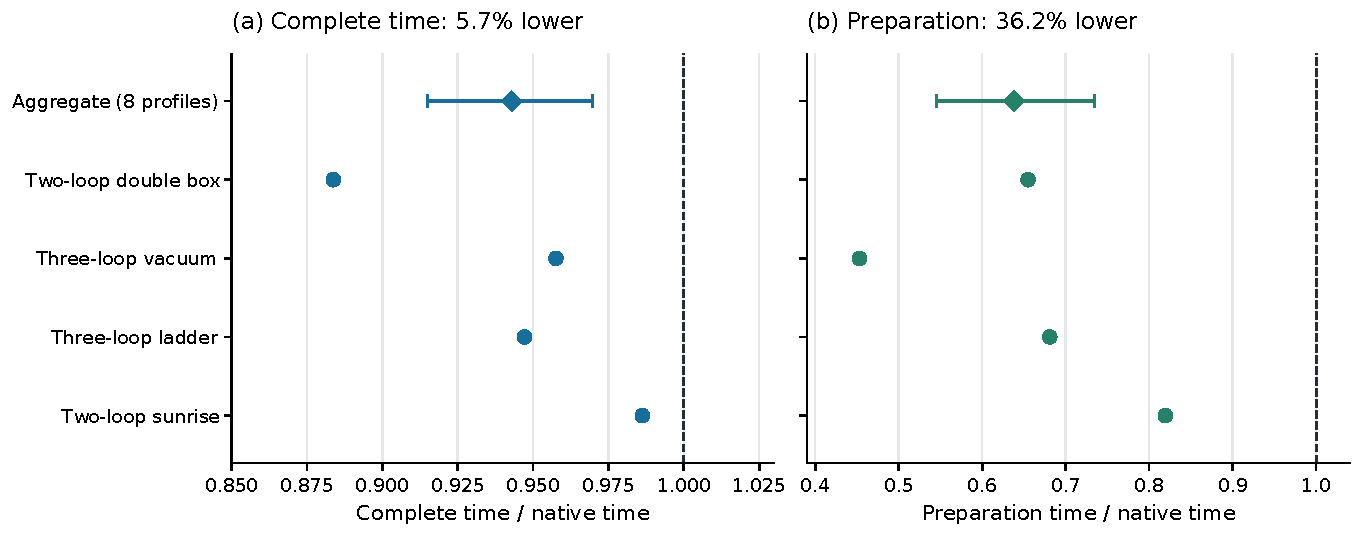
\includegraphics[width=\linewidth]{paper_figures/equation_results.pdf}
\caption{Equation selection saves more preparation time than complete reduction time. Each ratio compares the model with native choices in the same executable. The panels use different labelled ranges. The aggregate intervals describe variation across the eight profiles.}
\label{history:fig:equations}
\end{figure}

To test how far the original tree transfers, we also apply the fixed depth-twelve model to three structures absent from its training data: a massless nonplanar two-loop box, a massless pentagon, and a box with one external virtuality. Appendix~\ref{history:app:families} defines their propagators and invariants, using the massless limit of the nonplanar family in Ref.~\cite{KiraOriginal}. Four batches use rational kinematics and symbolic $d$. Three more keep the independent invariants symbolic, with coefficient fields $\Q(d,s,t)$, $\Q(d,s_{12},s_{23},s_{34},s_{45},s_{51})$, and $\Q(d,s,t,v)$. Here $s,t$ are four-point invariants, $s_{i,i+1}$ are adjacent five-point invariants, and $v$ is an external squared momentum.

The seven batches contain 88 targets and produce seventy comparison calculations. All final results pass exact checks, but every one of the 35 filtered calculations needs native fallback. The average time ratio is $1.252$, or 25.2\% more time. Checks cover 5,600 coefficient pairs, agreement with enlarged seed regions in all seven cases, and agreement after new rational substitutions in the three symbolic cases. The fallback therefore restores a correct answer at an additional cost. Figure~\ref{history:fig:transfer} records this transfer test before the new training described next.

\begin{figure}[tbp]
\centering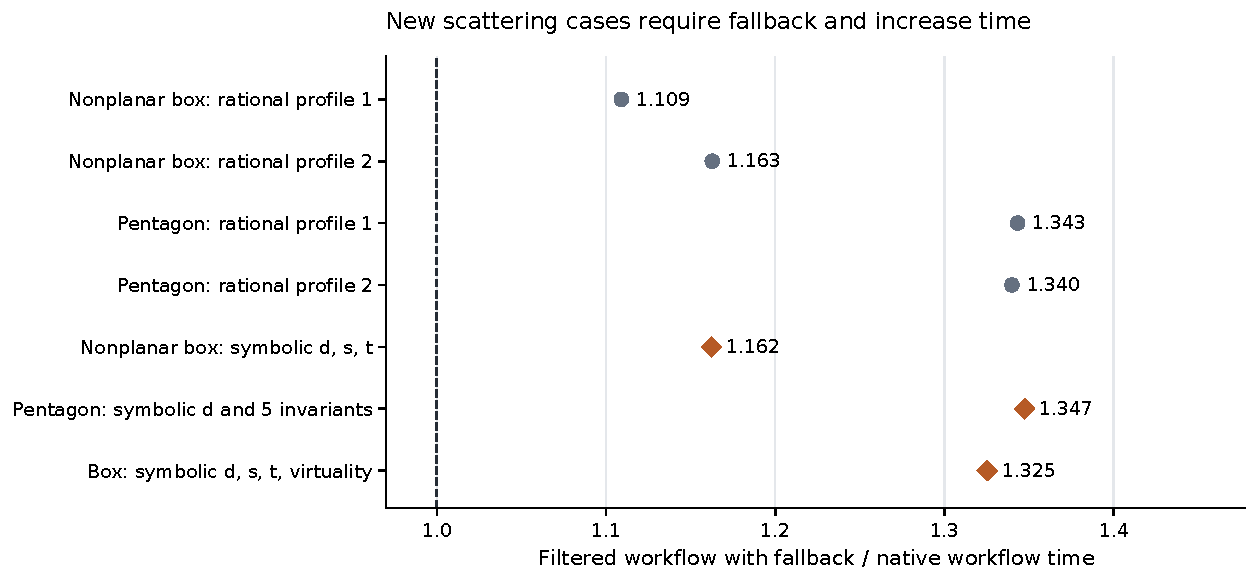
\includegraphics[width=\linewidth]{paper_figures/transfer_results.pdf}
\caption{The original equation model is slower on the new scattering structures. Each point compares five-run median times, including fallback. All 35 filtered calculations require a retry. This historical test uses the original weights, before additional training.}
\label{history:fig:transfer}
\end{figure}

\FloatBarrier
\providecommand{\StudySection}{\section}
\providecommand{\StudySubsection}{\subsection}

\StudySection{Training on the additional scattering structures}
\label{history:sec:adaptation}
The transfer failures raise a specific question: can examples from the missing structures teach a filter to retain enough equations? To test this, we train a new seed tree and equation tree for each of the nonplanar box, pentagon, and box with external virtuality. The original models remain fixed for comparison. Appendix~\ref{history:app:models} defines the new reference labels and tree fits.

Table~\ref{history:tab:scattering-split} separates the training, validation, and test batches. Rational batches use different invariant values in each split, while symbolic batches keep the independent invariants symbolic and use disjoint target lists. The graph structures occur in all three splits. Thus the test measures learning within these structures and separates that question from transfer to an unseen graph.

\begin{table}[!htbp]
\centering\small
\caption{The additional scattering study. Each of the three structures contributes equally to the batch counts.}
\label{history:tab:scattering-split}
\begin{tabular}{@{}lrrr@{}}\toprule
Part & Rational batches & Symbolic batches & Targets\\\midrule
Training & 6 & 3 & 108\\
Validation & 3 & 3 & 60\\
Testing & 6 & 3 & 108\\\bottomrule
\end{tabular}
\end{table}

Each tree has maximum depth twelve. The seed tree uses sixteen features and gives all operators of a seed the same score; the equation tree also receives the operator index, giving seventeen features and allowing different decisions for different operators. In both cases Kira enumerates its usual seed region, the tree filters candidates before coefficient construction, and native elimination remains active. These fits produce new trees trained on native reductions, while the original neural networks remain unchanged.

The fits use 59,706 equation records and 4,674 grouped seed records, including candidate patterns repeated in different training batches. Table~\ref{history:tab:scattering-fit} gives the tree sizes. Validation compares three score thresholds and fixes a setting before the reserved test. The four test methods are native choices, the original equation tree, the new seed tree, and the new equation tree. Five repetitions on identical targets give 180 calculations, with prediction, exact algebra, coefficient checks, cleanup, and fallback included in the timer. Reference discovery, training, and later recording of results are excluded.

\begin{table}[!htbp]
\centering\small
\caption{Additional training records and tree sizes. Each graph uses three training batches.}
\label{history:tab:scattering-fit}
\begin{tabular}{@{}lrrrr@{}}\toprule
Structure & Seed records & Seed nodes & Equation records & Equation nodes\\\midrule
Nonplanar box & 4,326 & 67 & 56,238 & 819 \\
Pentagon & 258 & 15 & 2,838 & 179 \\
Box with virtuality & 90 & 11 & 630 & 81 \\
\bottomrule
\end{tabular}
\end{table}

All 180 calculations pass exact checks of 9,880 returned coefficient entries. Eighteen additional applications receive the target and prescribed basis without reference coefficients, and their answers also pass an independent comparison after reduction. Each new selector completes all 45 timed attempts without fallback, whereas the original equation model needs fallback in all 45 trials. The new training therefore improves sufficiency on these inputs.

The timing result is more limited. Relative to native choices, the new seed model has ratio $1.027$ with descriptive 95\% interval $[0.995,1.086]$, and the new equation model has ratio $1.017$ with interval $[0.988,1.054]$. Their measured average times are 2.7\% and 1.7\% higher, respectively. The original filter has ratio $1.368$, or 36.8\% more time, on this new test. Its earlier 25.2\% overhead refers to different parameter points and symbolic targets. The additional training removes much of the fallback cost but does not establish an overall saving against native Kira.

\begin{table}[!htbp]
\centering\small
\caption{New reserved test results. Each value uses five repetitions. Ratios divide model time by native time; values below one are faster.}
\label{history:tab:scattering-time}
\begin{tabular}{@{}lrrrr@{}}\toprule
Case & Native (s) & Original tree & New seeds & New equations\\\midrule
Nonplanar box (13) & 4.163 & 1.293 & 1.023 & 0.980 \\
Nonplanar box (14) & 4.140 & 1.221 & 1.002 & 0.974 \\
Nonplanar box (symbolic) & 4.458 & 1.233 & 0.983 & 1.010 \\
Pentagon (13) & 1.005 & 1.439 & 0.963 & 1.016 \\
Pentagon (14) & 0.965 & 1.436 & 1.069 & 1.038 \\
Pentagon (symbolic) & 1.120 & 1.356 & 0.958 & 0.979 \\
Box with virtuality (13) & 0.826 & 1.339 & 0.953 & 0.991 \\
Box with virtuality (14) & 0.763 & 1.529 & 1.152 & 1.124 \\
Box with virtuality (symbolic) & 0.729 & 1.499 & 1.166 & 1.052 \\
\midrule
Geometric mean ratio & --- & 1.368 & 1.027 & 1.017\\\bottomrule
\end{tabular}
\end{table}

The individual results in Table~\ref{history:tab:scattering-time} and Figures~\ref{history:fig:adapted-time}--\ref{history:fig:adapted-sufficiency} explain this distinction. Some new filters reduce time, while others add overhead to cases that native Kira already solves quickly. We therefore retain native choices as the default for this scattering study. The result supports training on the missing structures to improve sufficiency, although it cannot isolate missing data as the sole cause of the original failure: the study also changes the seed-model architecture and fits separate trees for each graph. The intervals resample the three graph groups and describe this limited comparison.

\begin{figure}[tbp]
\centering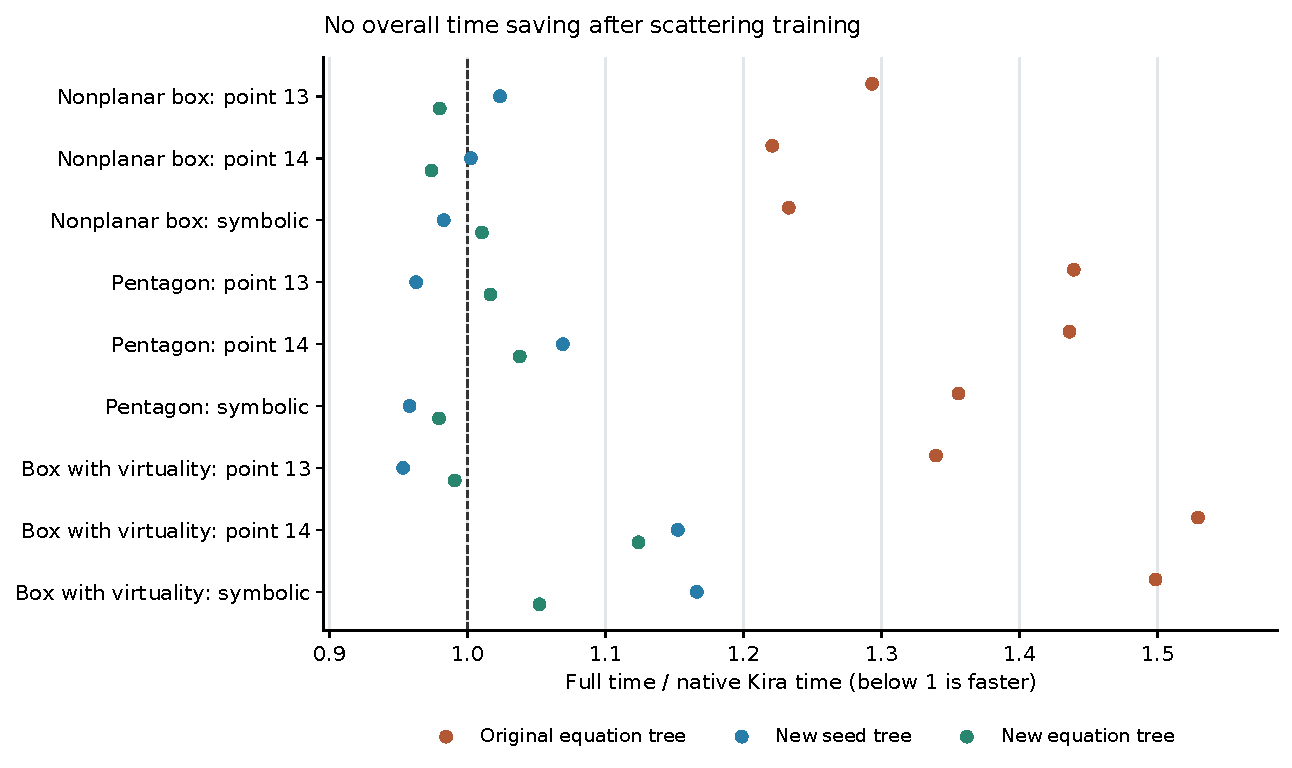
\includegraphics[width=\linewidth]{paper_figures/scattering_training.pdf}
\caption{Training on the three structures removes much of the original filter's overhead, but gives no overall saving against native Kira. Points compare five-run median complete times, including prediction, checks and fallback. The dashed line marks equal time. No per-case uncertainty interval is inferred from five repetitions.}
\label{history:fig:adapted-time}
\end{figure}

\begin{figure}[tbp]
\centering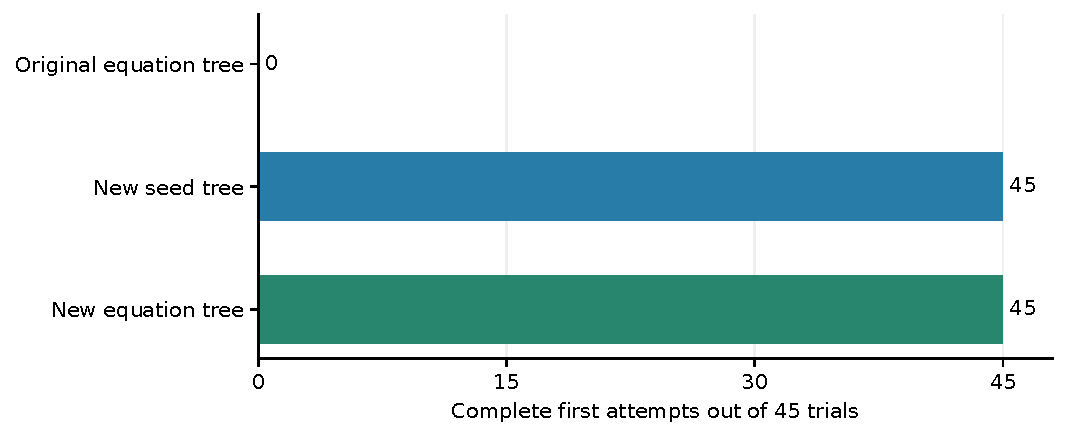
\includegraphics[width=.85\linewidth]{paper_figures/scattering_sufficiency.pdf}
\caption{The new selectors provide sufficient equations on every first attempt. Each method has 45 trials across nine batches. Native fallback lets the original filter eventually complete, and its added time remains in the comparison above.}
\label{history:fig:adapted-sufficiency}
\end{figure}

\FloatBarrier


\subsection{IBP relations and exact elimination}
\label{history:app:ibp}
This appendix derives the identities and row operations used throughout the study. For a seed $\boldsymbol\sigma$, write its denominator product as $P_{\boldsymbol\sigma}=\prod_iD_i^{-\sigma_i}$ and define $\partial_k^\mu=\partial/\partial\ell_{k\mu}$. The product rule separates the derivative in Eq.~\eqref{history:eq:ibp} into a derivative of the momentum vector and a derivative of the propagator factors:
\begin{align}
 \partial_k^\mu(v_\mu P_{\boldsymbol\sigma})
 &= (\partial_k\cdot v)P_{\boldsymbol\sigma}
       +v\cdot\partial_k P_{\boldsymbol\sigma},\\
 v\cdot\partial_k P_{\boldsymbol\sigma}
 &=-\sum_i\sigma_i(v\cdot\partial_kD_i)
       D_i^{-\sigma_i-1}\prod_{j\ne i}D_j^{-\sigma_j}.
 \label{history:eq:ibp-expanded}
\end{align}
When $v=\ell_h$, the first derivative is $\partial_k\cdot v=d\delta_{kh}$, where $\delta_{kh}$ equals one for $k=h$ and zero otherwise; for an external momentum it vanishes. The integrated total derivative is zero in a region of convergence, and analytic continuation extends the relation to dimensional regularization~\cite{ChetyrkinTkachov,Weinzierl2022}. The same regularization prescription sets scaleless integrals to zero.

With a complete scalar-product basis, the scalar numerator $v\cdot\partial_kD_i$ can be written as $u_i+\sum_j v_{ij}D_j$. The coefficients $u_i$ and $v_{ij}$ depend on masses, invariants and the chosen momentum routing. Substituting in Eq.~\eqref{history:eq:ibp-expanded} gives
\begin{equation}
 0=\delta_v I_{\boldsymbol\sigma}
 -\sum_i\sigma_i u_i I_{\boldsymbol\sigma+\boldsymbol e_i}
 -\sum_{i,j}\sigma_i v_{ij}
       I_{\boldsymbol\sigma+\boldsymbol e_i-\boldsymbol e_j},
 \label{history:eq:ibp-shifts}
\end{equation}
Here $\delta_v=\partial_k\cdot v$, and the unit vector $\boldsymbol e_i$ increases index $i$ by one. The derivative therefore relates the seed integral to integrals with shifted integer indices. Auxiliary denominators complete an otherwise incomplete scalar-product representation. When the denominator representation is dependent, additional algebraic relations are needed; the restricted vacuum family in Appendix~\ref{history:app:vacuum} uses explicit mass partial fractions.

Suppose row $q$ of such a system satisfies $\sum_jA_{qj}I_j=0$ and $A_{qk}\ne0$. Solving this row for the pivot integral gives
\begin{equation}
 I_k=-\sum_{j\ne k}\frac{A_{qj}}{A_{qk}}I_j.
 \label{history:eq:pivot}
\end{equation}
For a second identity row, or a target coefficient row $r$, subtract $(A_{rk}/A_{qk})$ times the zero identity. The resulting coefficients are
\begin{equation}
 A'_{rj}=A_{rj}-\frac{A_{rk}}{A_{qk}}A_{qj},
 \qquad A'_{rk}=0.
 \label{history:eq:row}
\end{equation}
Because the subtracted identity is zero, this operation preserves the target while removing its pivot entry. Choosing a different allowed source row can change the intermediate expressions and their cost without changing that equality. Repeated elimination removes the nonmaster columns and yields Eq.~\eqref{history:eq:master}, provided each pivot coefficient is nonzero. Kinematic points at which a required denominator vanishes require a separate calculation.

\subsection{Reverse construction and the meaning of reference labels}
\label{history:app:construction}
The reverse construction provides targets with known answers because each checked source identity $E_q$ is a linear combination of integrals that equals zero. Substituting these identities into Eq.~\eqref{history:eq:reverse} gives
\begin{equation}
 T-\sum_mr_mM_m=\sum_q\lambda_qE_q=0.
 \label{history:eq:reverse-check}
\end{equation}
The equality fixes the master coefficients of the constructed expression. Expanding the source identities and collecting terms with equal index vectors then gives the target supplied to the model. Recording the operations, source rows, and seed--operator labels provides a path back to the masters. The coefficients $\lambda_q$ and $r_m$ may be rational functions, including constants as a special case. Algebraic mass partial-fraction identities are recorded separately because they have no IBP seed label.

Different zero identities can give different construction histories for the same target. A saved seed set is therefore sufficient, but need not be unique or smallest. Likewise, the saved row sequence need not use the fewest operations. A seed label records membership in one checked set, and a row label records the next step in one checked path. The final master coefficients and later steps do not enter the model inputs.

\subsection{Model specification and training objectives}
\label{history:app:models}
This appendix specifies what each model learns and how its training objective is obtained. We begin with the seed network, whose symbolic target coefficients must first be represented by numerical inputs. We split each expression into tokens and count individual tokens and consecutive pairs and triples. A fixed signed map places these counts in 64 components. Different token groups can share a component, so equal representations do not prove equal expressions. Integral indices, complexity counts and term positions give further inputs. A shared hyperbolic-tangent map converts each term into a vector $\boldsymbol h_u\in\mathbb R^{32}$. Family symbols, master indices and candidate indices give separate 32-component vectors.

\subsubsection{Seed representation and loss}
The target representation includes the following summary of ordered term pairs:
\begin{equation}
 \boldsymbol h_{\rm pair}=
 \frac{1}{n_T(n_T-1)}\sum_{u\ne v}
 \psi_\theta([\boldsymbol h_u,\boldsymbol h_v,
       \boldsymbol h_u-\boldsymbol h_v,
       \boldsymbol h_u\odot\boldsymbol h_v]),
 \label{history:eq:pair}
\end{equation}
where $n_T$ is the number of terms, square brackets concatenate vectors, $\odot$ multiplies components and $\psi_\theta$ returns 32 components. For $n_T=1$, the summary is zero. This definition covers ordered pairs, not all larger term subsets. The candidate vector $\boldsymbol u_b$ weights target terms through scaled dot-product attention~\cite{AttentionIsAllYouNeed}:
\begin{equation}
 w_{bu}=\frac{\exp(\boldsymbol u_b\cdot\boldsymbol h_u/\sqrt{32})}
 {\sum_v\exp(\boldsymbol u_b\cdot\boldsymbol h_v/\sqrt{32})},
 \qquad \boldsymbol v_b=\sum_u w_{bu}\boldsymbol h_u.
\end{equation}
The final input combines the mean and componentwise maximum of the term vectors with the pair, family, basis, seed, and attention-weighted term vectors. A hidden layer with 64 components produces $g_\theta$ in Eq.~\eqref{history:eq:seed}. Shared maps and aggregation follow Ref.~\cite{DeepSets}, while stored positions retain the target term order. Reordering the candidate seeds changes only the order of the output scores.

If $y_b\in\{0,1\}$ is recorded seed membership, a Bernoulli model assigns label likelihood $p_b^{y_b}(1-p_b)^{1-y_b}$. Taking its negative logarithm gives $-y_b\log p_b-(1-y_b)\log(1-p_b)$. Averaging within each candidate list and then across targets gives the implemented loss
\begin{equation}
 \mathcal L_s=-\frac{1}{|\mathcal D_s|}\sum_{T\in\mathcal D_s}
 \frac{1}{|\Cset(T)|}\sum_{b\in\Cset(T)}
 [y_b\log p_b+(1-y_b)\log(1-p_b)].
 \label{history:eq:seed-loss}
\end{equation}
Here $\mathcal D_s$ is the training-target set. This objective treats each target equally and does not claim that true seed dependencies are statistically independent. Training uses AdamW~\cite{AdamW} with learning rate $10^{-3}$, weight decay $10^{-4}$, gradient norm limit one and up to 32 targets per update. The threshold $1/2$ stays fixed during the expanded label test.

\subsubsection{Row representation and loss}
The row network compares the actions available at the current matrix state. Let $\mathcal A$ be that action list, and let $\boldsymbol f_a\in\mathbb R^{132}$ be the feature vector for action $a$. The encoder is $\boldsymbol h_a=\tanh(W\boldsymbol f_a+\boldsymbol b)$ with 32 components. Concatenating $\boldsymbol h_a$ with the mean and componentwise maximum over $\mathcal A$ gives the input to a 64-component hidden layer. Its scalar output $g_a$ defines
\begin{equation}
 p(a\mid A,\mathcal A)=\frac{e^{g_a}}{\sum_{b\in\mathcal A}e^{g_b}},
 \qquad
 \mathcal L_r=-\frac{1}{|\mathcal D_r|}
       \sum_{(A,\mathcal A,a^*)\in\mathcal D_r}\log p(a^*\mid A,\mathcal A).
 \label{history:eq:row-loss}
\end{equation}
Here $A$ is the matrix, $a^*$ is the recorded action, and $\mathcal D_r$ contains the training states with a choice. The softmax denominator normalizes the probabilities to one, and taking the negative logarithm of the recorded action's probability gives the loss. A state with one action has zero loss. Training uses the seed model's AdamW settings and 256 states per update. Trial updates modulo a prime provide cancellation features. The numerical size of a modular value does not measure the size of a real coefficient.

Later row models learn the cost of an action. One fit predicts the logarithm of the measured insertion time. Another counts the remaining forward insertions after that action, with Kira choosing later steps. If insertion $j$ uses $n_j$ source entries, its estimated cost is $1+2n_j$: one division, followed by a multiplication and subtraction for each entry. Thus the cost label is $C(S,q)=\sum_j(1+2n_j)$ for state $S$ and choice $q$. The later tree fits
\begin{equation}
 y_q=\frac{C(S,q)-C(S,0)}{\max\{1,\max_b C(S,b)-\min_b C(S,b)\}},
 \qquad \widehat y_q=h(\boldsymbol x_q-\boldsymbol x_0),
\end{equation}
where $0$ denotes Kira's native source and $\boldsymbol x_q$ contains eighteen current-row and overlap features. Weighted squared error gives each training family equal weight. Validation selects the tree and the required predicted improvement, and exact coefficients must agree before a measured continuation enters training. This count describes coefficient operations, while complete timings include the algebraic work inside each coefficient operation. Neither training objective proves a globally minimum path.

\subsubsection{Equation features and tree fitting}
The equation model uses a reference label derived from the support of an equation, meaning the set of integrals with nonzero coefficients. An equation label records whether this support appears in Kira's selected system. Table~\ref{history:tab:features} groups the equation tree's seventeen inputs. They describe the seed and target before symbolic coefficient construction. For seed indices $\boldsymbol\sigma$ and target indices $\boldsymbol a$, the distance is $\sum_i|\sigma_i-a_i|$. The additional-power count is $\sum_i\max(\sigma_i-1,0)$, and the numerator rank is $\sum_i\max(-\sigma_i,0)$. Neither quantity requires equation coefficients.

\begin{table}[!htbp]
\centering\small
\caption{Inputs to the original equation tree. The scattering seed trees omit the operator input and use sixteen features.}
\label{history:tab:features}
\begin{tabularx}{\linewidth}{@{}lYr@{}}\toprule
Group & Quantities & Number\\\midrule
Family and request & Loops, external momenta, index count, logarithm of target count & 4\\
Seed & Positive indices, additional powers, numerator rank & 3\\
Target limits & Excess seed powers and rank above target maxima & 2\\
Sector & Whether requested; excess powers and rank above its target maxima & 3\\
Target distance & Minimum index distance; whether the seed is a target & 2\\
Operator & IBP operator index & 1\\
Overall limits & Maximum target powers and numerator rank & 2\\\bottomrule
\end{tabularx}
\end{table}

Training gives each physical profile equal total weight by assigning each row weight $1/(n_b B_g)$, where $n_b$ is its batch size and $B_g$ is the number of training batches in its profile. At a node, let $w_+,w_-$ be the positive and negative total weights. Half the weighted binary Gini impurity is
\begin{equation}
 H=\frac{w_+w_-}{w_++w_-}.
\end{equation}
Indeed, with $p=w_+/(w_++w_-)$, the weighted Gini expression is $(w_++w_-)[1-p^2-(1-p)^2]=2H$. Each proposed split reduces $H$ by the sum of its two children's values. The fit tests 25 feature quantiles between 0.02 and 0.98, rejects children below the stated population limit, and selects the largest positive reduction. This is the classification-tree construction of Ref.~\cite{CART1984} with our bounded set of candidate splits.

A leaf with $n_+$ positive rows among $n$ rows returns
\begin{equation}
 p_{\rm leaf}=\frac{n_++1/2}{n+1}.
\end{equation}
Adding one half-count to each class gives a finite score even when a leaf contains only one class. The original tree keeps an equation when $p_{\rm leaf}\geq0.01$. These scores estimate reference-set membership; they are not calibrated probabilities that the whole reduction succeeds. The depth-eight and depth-twelve fits require at least 24 and eight rows in each child. The split procedure follows Ref.~\cite{CART1984}. A basis check and fallback still test whether the selected system is sufficient.

\subsubsection{Additional scattering seed and equation trees}
The added scattering study fits a separate pair of trees for each of the three graph structures. The equation labels use the same selected-support rule as the original equation model. Let $y_{\sigma,o}$ be one when the native selected system contains the recorded equation support for seed $\sigma$ and operator $o$. A seed receives label one when any of its operators has label one:
\begin{equation}
 y_\sigma=\max_o y_{\sigma,o}.
 \label{history:eq:adapted-seed-label}
\end{equation}
For binary labels, this maximum is one exactly when at least one selected-support equation comes from the seed. This proves the stated membership rule. The label gives a useful reference set, not a proof that every labelled seed is necessary.

Each seed appears once per training batch. Its tree uses the sixteen features that do not depend on the operator. Thus every operator of that seed receives the same score. The early filter either permits or skips construction of all its equations. Kira still enumerates the seed region and applies its native symmetries. The equation tree uses all seventeen features and can keep different operators of the same seed.

Both fits have maximum depth twelve and at least eight records in each child. Each training batch has equal total weight. The split rule and leaf score are those derived above. Validation compares thresholds $0.001$, $0.01$ and $0.05$ using full reduction time. Three repetitions contribute to each validation median. The chosen threshold minimizes the geometric mean ratio over the rational and symbolic validation batches of its graph. Model parameters and thresholds are fixed before testing. For the nonplanar box, both thresholds are $0.05$. For the pentagon, the seed and equation thresholds are $0.05$ and $0.001$. For the box with virtuality, they are $0.001$ and $0.01$. These fits create new small tree models; they do not change the original neural checkpoints. The reserved timing test gives no overall saving, so the application keeps native choices as its default.

\subsection{Exact reuse for the restricted vacuum family}
\label{history:app:vacuum}\label{app:vacuum}
The large cumulative saving in Section~\ref{history:sec:overall} follows from exact recurrences in a particular Euclidean vacuum family. We derive them here to state both the source of the saving and the restrictions on its use. The family has positive, distinct squared masses $\mu_j=\rho_j\mu$:
\begin{equation}
 V^{(L)}_{\boldsymbol b}=
 \int\prod_{h=1}^L\frac{d^d\ell_h}{\pi^{d/2}}
 \frac{1}{\ell_1^2\cdots\ell_L^2}
 \prod_{j=1}^{R}(Q^2+\mu_j)^{-b_j},
 \qquad Q=\sum_{h=1}^L\ell_h.
 \label{history:eq:vacuum}
\end{equation}
Here $b_j$ is a nonnegative integer, $B=\sum_jb_j\geq1$, $R$ is the number of massive denominators, $\mu$ is a common squared-mass scale and $\rho_j$ is a positive mass ratio. Each massless denominator has power one. All massive denominators share $Q$, so this family has special algebraic dependencies. Its prescribed masters are $M_j^{(L)}=V^{(L)}_{\boldsymbol e_j}$. The comparison uses $R=2,3,4$ and $\mu=1$ in the selected units.

\subsubsection{Euler and mass partial-fraction identities}
We first derive two relations that lower the massive propagator powers. Let $f$ be the integrand without the measure. The simultaneous Euler derivative gives $\sum_h\ell_h\cdot\partial_{\ell_h}(\ell_i^2)^{-1}=-2(\ell_i^2)^{-1}$ for each massless factor. Also, $\sum_h\ell_h\cdot\partial_{\ell_h}Q^2=2Q^2$. Therefore
\begin{equation}
 \sum_h\partial_{\ell_h}\cdot(\ell_h f)
 =\left[Ld-2L-2\sum_jb_j\frac{Q^2}{Q^2+\mu_j}\right]f.
\end{equation}
Use $Q^2=(Q^2+\mu_j)-\mu_j$ and integrate the derivative as in Appendix~\ref{history:app:ibp}. This gives
\begin{equation}
 0=[L(d-2)-2B]V^{(L)}_{\boldsymbol b}
       +2\sum_j b_j\mu_jV^{(L)}_{\boldsymbol b+\boldsymbol e_j}.
 \label{history:eq:euler-vac}
\end{equation}
For two present massive denominators, the integrand identity
$(Q^2+\mu_i)-(Q^2+\mu_j)=\mu_i-\mu_j$ separately gives
\begin{equation}
 (\mu_i-\mu_j)V_{\boldsymbol b}^{(L)}
   =V_{\boldsymbol b-\boldsymbol e_i}^{(L)}
    -V_{\boldsymbol b-\boldsymbol e_j}^{(L)}.
 \label{history:eq:mass-vac}
\end{equation}
This second relation is an algebraic partial fraction, so it introduces no additional IBP seed.

\subsubsection{A recurrence shared across loop orders}
To make the common loop dependence explicit, define $z=L(d-2)$ and $W_{\boldsymbol b}^{(L)}=\mu^{B-1}V_{\boldsymbol b}^{(L)}$. Multiplication by this power of $\mu$ gives $W$ the same mass dimension as the masters. Substituting in Eqs.~\eqref{history:eq:euler-vac} and \eqref{history:eq:mass-vac} removes the common scale. If $\boldsymbol C_{\boldsymbol b}(z)$ is the vector of master coefficients of $W_{\boldsymbol b}^{(L)}$, then
\begin{align}
 \boldsymbol C_{\boldsymbol b}(z)
 &=\frac{\boldsymbol C_{\boldsymbol b-\boldsymbol e_i}(z)
          -\boldsymbol C_{\boldsymbol b-\boldsymbol e_j}(z)}{\rho_i-\rho_j},
       &&b_i,b_j>0,\label{history:eq:mass-rec}\\
 \boldsymbol C_{k\boldsymbol e_j}(z)
 &=\frac{2(k-1)-z}{2(k-1)\rho_j}
         \boldsymbol C_{(k-1)\boldsymbol e_j}(z),
       &&k\geq2.\label{history:eq:euler-rec}
\end{align}
The initial vector is $\boldsymbol C_{\boldsymbol e_j}=\boldsymbol e_j$. Every recurrence lowers $B$, so it terminates at the prescribed masters. Its coefficients depend on $L$ only through $z$. Induction on $B$ shows that they are polynomials in $z$ with rational coefficients at fixed rational $\rho_j$. One calculation can therefore supply all requested loop orders by substituting $z=L(d-2)$.

\subsubsection{An independent coefficient check}
The recurrence result is checked by obtaining the mixed-denominator coefficients through a Taylor partial-fraction expansion. For a dimensionless auxiliary variable $x$, write
\begin{equation}
 \prod_i(x+\rho_i)^{-b_i}
   =\sum_{j:b_j>0}\sum_{k=1}^{b_j}\frac{a_{jk}}{(x+\rho_j)^k}.
\end{equation}
At the pole $x=-\rho_j$, set $t=x+\rho_j$. Multiplying by $t^{b_j}$ and expanding the regular factors shows that the principal-part coefficient is
\begin{equation}
 a_{jk}=[t^{b_j-k}]\prod_{i\ne j}(\rho_i-\rho_j+t)^{-b_i}.
 \label{history:eq:taylor}
\end{equation}
Here $[t^n]$ extracts Taylor coefficient $n$ and factors with $b_i=0$ are one. Applying Eq.~\eqref{history:eq:euler-rec} repeatedly to each pole term gives
\begin{equation}
 C_{\boldsymbol b j}(z)=\sum_{k=1}^{b_j}a_{jk}
       \prod_{h=1}^{k-1}\frac{2h-z}{2h\rho_j},
 \qquad
 V^{(L)}_{\boldsymbol b}
 =\mu^{1-B}\sum_j C_{\boldsymbol b j}(L(d-2))M_j^{(L)}.
 \label{history:eq:checked-vacuum}
\end{equation}
An empty product is defined as one. This Taylor calculation checks every returned polynomial coefficient before the substitution for $z$ and does not follow the chosen sequence of pair recurrences. The derivation requires distinct $\rho_j$, unit powers for the massless propagators, and the shared momentum $Q$. These assumptions delimit the family to which the result applies.

\subsection{Measurement definitions and comparison conditions}
\label{history:app:timing}
The comparisons use separate measures for label prediction, algebraic completion, and elapsed time. For the label measures, let TP be the number of selected reference seeds, FP the number of selected seeds absent from the reference set, and FN the number of omitted reference seeds. Precision is $P=\mathrm{TP}/(\mathrm{TP}+\mathrm{FP})$ and recall is $R=\mathrm{TP}/(\mathrm{TP}+\mathrm{FN})$. Defining $F_1$ as their harmonic mean gives
\begin{equation}
 F_1=\frac{2}{P^{-1}+R^{-1}}=\frac{2PR}{P+R}
     =\frac{2\mathrm{TP}}{2\mathrm{TP}+\mathrm{FP}+\mathrm{FN}}.
\end{equation}
Complete-set agreement counts targets for which the entire predicted seed set equals the recorded set. Algebraic sufficiency instead counts targets that reach the prescribed master basis using the selected equations. Since a target can have several sufficient seed sets, these measures need not agree with each other or with the individual-label scores in Figure~\ref{history:fig:seed}.

For timing, let $T_{abr}$ be the measured time for method $a$, batch $b$ and repetition $r$. We use $\widetilde T_{ab}=\operatorname{median}_{r=1,\ldots,5}T_{abr}$. For the later native comparisons, if physical group $g$ contains batches $B_g$, define the equal-group mean logarithmic ratio
\begin{equation}
 \overline\ell=\frac1G\sum_{g=1}^G\frac1{|B_g|}
 \sum_{b\in B_g}\log\frac{\widetilde T_{ab}}{\widetilde T_{cb}},
 \qquad R_{a/c}=e^{\overline\ell}.
 \label{history:eq:ratio}
\end{equation}
Here $c$ identifies the control and $G$ is the number of physical groups. Exponentiating the mean log ratio gives the geometric mean; ratios below one indicate lower time. Reversing numerator and denominator changes $\overline\ell$ to $-\overline\ell$, so speedup is $S=1/R_{a/c}$ and the time reduction is $100(1-R_{a/c})\%$. The cumulative study uses one batch per group. The supplied-equation seed comparison instead gives each complete paired batch equal weight; its interval resamples six related kinematic groups. Following bootstrap resampling~\cite{Efron1979}, reported descriptive 95\% intervals resample complete groups 10,000 times while retaining paired methods and repetitions. They describe case-to-case variation in these experiments. We do not infer new uncertainty intervals for figures whose source summaries provide only point estimates.

The supplied-equation seed test includes target preparation, inference, early basis checking, reduction, result checking and fallback. It excludes original IBP-pool generation. It rotates methods within each family and target batch on the same node, and includes only complete paired batches in its ratio summary while preserving incomplete and skipped trials in the accounting.

The native equation and transfer tests include input preparation, model loading and evaluation, Kira startup, native IBP generation, elimination, basis and coefficient checks, cleanup and every fallback. Independent reference discovery and the later independent check lie outside the timer. In the equation test, the native and learned arms receive the same executable-level improvements. The eight reserved profiles test new masses and invariants within known structures; the seven transfer cases additionally test new structures and symbolic invariants.

The cumulative test includes fresh-worker startup, input loading, supplied Euler and mass-identity construction, algebra, verification, output saving and complete output reading. Eight groups use maximum massive powers 8, 10, 12 or 14, with two groups at each bound. They request 16, 32, 48 or 64 targets per profile, capped by availability. Each group contains three mass profiles and all loop orders 1--12. Paired methods use the same resources, and their order changes between repetition blocks. Each method recomputes the reduction. Waiting for resources, offline training and the later independent check remain outside all reported production times.

The initial live-matrix comparison uses three repetitions of four methods on seven physical cases, giving 84 workflows. Its complete ratio is the geometric mean of the seven paired median ratios and carries no reported uncertainty interval. The later native implementation comparison uses five repetitions and sixteen batches; it repeats earlier physical profiles to measure the implementation change.

The reported numbers are measurements from this study. We keep the original label tests, seed tests, row tests, equation tests, scattering tests and vacuum benchmark separate. This prevents differences in targets or timed work from being mistaken for a combined model gain. The archived notes preserve earlier experiments, including negative results.

\subsection{Integral families and kinematic conventions}
\label{history:app:families}
The physical scope of each test is determined by its denominator momenta, masses, and external scalar products. This appendix gives those definitions for the training and test families. Together with an index vector, or a rational linear combination of index vectors in one family, they specify the targets without requiring an individual listing of the full collection. Unless stated otherwise, $D_i=q_i^2-m_i^2+i0$ and the measure is that of Eq.~\eqref{history:eq:family}. The Euclidean vacuum family keeps the sign convention in Eq.~\eqref{history:eq:vacuum}.

\subsubsection{Initial one-loop and two-loop families}
For the one-loop tadpole, $q_1=\ell$ and $m_1^2=\mu>0$. For the bubbles,
\begin{equation}
 \boldsymbol q=(\ell,\ell-p),\qquad p^2=s,
 \qquad (m_1^2,m_2^2)\in\{(0,0),(\mu,0),(\mu,\mu),(\mu_1,\mu_2)\}.
\end{equation}
The symbols $\mu,\mu_1,\mu_2$ denote squared masses, with $\mu_1\ne\mu_2$ in the unequal-mass case. The triangle routing is
\begin{equation}
 \boldsymbol q=(\ell,\ell-p_1,\ell-p_1-p_2),\qquad
 (p_1^2,p_2^2,(p_1+p_2)^2)=(u_1,u_2,u_3).
\end{equation}
Expanding $(p_1+p_2)^2$ gives $2p_1\cdot p_2=u_3-u_1-u_2$. Three massless triangle classes use virtualities $(0,0,s)$, $(0,u_2,u_3)$ and $(u_1,u_2,u_3)$. Two equal-mass classes, with all internal squared masses $\mu$, use $(0,0,s)$ and $(u_1,u_2,u_3)$. Each displayed nonzero virtuality is independent at generic kinematics.

The initial massless boxes use four incoming external momenta, $p_4=-p_1-p_2-p_3$, and
\begin{equation}
 \boldsymbol q=(\ell,\ell-p_1,\ell-p_1-p_2,\ell-p_1-p_2-p_3),
 \quad s=(p_1+p_2)^2,\quad t=(p_2+p_3)^2.
\end{equation}
Writing $u_i=p_i^2$, the three classes have $(u_1,u_2,u_3,u_4)=(0,0,0,0)$, $(0,0,0,u_4)$ and $(u_1,u_2,u_3,u_4)$. Expanding the definitions of $s,t$ and $p_4^2$ gives
\begin{equation}
 2p_1\cdot p_2=s-u_1-u_2,\quad
 2p_2\cdot p_3=t-u_2-u_3,\quad
 2p_1\cdot p_3=u_4+u_2-s-t.
\end{equation}
These definitions give thirteen one-loop classes. The initial two-loop massless two-point family uses
\begin{equation}
 \boldsymbol q=(\ell_1,\ell_2,\ell_1-\ell_2,\ell_1-p,\ell_2-p),
 \qquad p^2=s,\qquad m_i^2=0.
\end{equation}
The equal-mass sunrise uses $\boldsymbol q=(\ell_1,\ell_2,p-\ell_1-\ell_2,p-\ell_1,p-\ell_2)$, with masses $(\mu,\mu,\mu,0,0)$ and $p^2=s$. Its last two entries are auxiliary: $a_4,a_5\leq0$. The equal-mass vacuum sunset has $\boldsymbol q=(\ell_1,\ell_2,\ell_1-\ell_2)$ and all three squared masses $\mu$. These three classes complete the initial sixteen. Their subsectors include the integrals obtained by removing physical denominators.

\subsubsection{Additional one-loop mass and invariant assignments}
The 984 added box families use a more general assignment than the three initial massless boxes:
\begin{equation}
 D_i=(\ell-Q_i)^2-\mu_{\alpha_i}+i0,
 \quad Q_1=0,\quad \mu_0=0,\quad \alpha_i\in\{0,1,2,3\}.
\end{equation}
The nonzero squared masses $\mu_1,\mu_2,\mu_3$ are independent. Repeated labels impose equal masses. The three external shifts $Q_2,Q_3,Q_4$ have squared differences
\begin{equation}
 \Delta_{ij}=(Q_i-Q_j)^2=y_{\beta_{ij}},
 \quad y_0=0,\quad \beta_{ij}\in\{0,1,2,3\}.
\end{equation}
The nonzero $y_1,y_2,y_3$ are independent invariants. Expanding a squared difference gives the Gram matrix
\begin{equation}
 Q_i\cdot Q_j=\frac{\Delta_{1i}+\Delta_{1j}-\Delta_{ij}}2,
 \qquad i,j\in\{2,3,4\}.
\end{equation}
The construction rejects singular sampled Gram matrices and identifies assignments related by propagator permutations or by relabelling nonzero masses and invariants. A fixed order selects 984 of 1,673 admissible inequivalent profiles after excluding the original massless boxes. This extends the initial collection to 1,000 families with 9,678 family-local masters and 240,472 targets before the higher-loop additions. Each profile gives a symbolic family through its zeros and equality conditions. The single-target seed timing comparison uses twelve reserved instances of these boxes. Its targets follow the reverse construction in Appendix~\ref{history:app:construction}, rather than the native target enumeration below.

\subsubsection{Native multiloop comparisons}
The sunrise comparisons allow independent masses on the same three physical propagators. The other native comparison families use
\begin{align}
 \boldsymbol q_{\rm DB}={}&(\ell_1,\ell_1-p_1,\ell_1-p_1-p_2,
 \ell_2,\ell_2-p_1-p_2,\ell_2-p_1-p_2-p_3,\nonumber\\
 &\ell_1-\ell_2,\ell_1-p_3,\ell_2-p_1),\\
 \boldsymbol q_{\rm V}={}&(\ell_1,\ell_2,\ell_3,\ell_1-\ell_2,
 \ell_2-\ell_3,\ell_1-\ell_3),\\
 \boldsymbol q_{\rm L}={}&(\ell_1,\ell_1-p,\ell_2,\ell_2-p,\ell_3,
 \ell_3-p,\ell_1-\ell_2,\ell_2-\ell_3,\ell_1-\ell_3).
\end{align}
The double box has two loops and seven physical denominators; its last two entries are auxiliary. The vacuum has three loops and six physical denominators. The ladder has three loops and eight physical denominators; its last entry is auxiliary. Auxiliary indices remain nonpositive. The massless double box has $p_i^2=0$ and uses $2p_1\cdot p_2=s$, $2p_1\cdot p_3=t$, $2p_2\cdot p_3=-s-t$. This local definition of $t$ differs from the initial box convention because the routing differs.

For the final early-equation test, the sunrise squared-mass vectors are $(2,7,11)$ and $(3,7,13)$, with $p^2=-101,-103$. The double-box profiles are $(s,t)=(-101,-103),(-107,-109)$. The vacuum squared-mass vectors are $(1,1,1,1,1,11)$ and $(1,1,1,13,13,13)$. The ladder has squared masses $(1,0,0,0,0,0,0,0)$ and $p^2=-101,-103$. All values use a common squared-momentum unit. These choices keep $d$ symbolic and give coefficients in $\Q(d)$.

The target order starts with the full-sector corner, then adds each single extra propagator power and each available single auxiliary numerator. The construction repeats after removing one, two and three physical denominators, retains at least two, and removes duplicates. The comparison takes 21 sunrise targets and batches of 32 and 128 targets for each other profile. This gives the fourteen batches in Section~\ref{history:sec:equations}.

\subsubsection{New scattering structures and symbolic invariants}
The massless nonplanar box uses the routing of Ref.~\cite{KiraOriginal}:
\begin{align}
 \boldsymbol q_{\rm NP}={}&(\ell_1,\ell_2,p_1-\ell_1,p_2-\ell_2,
 p_1+p_2-p_3-\ell_1,\nonumber\\
 &p_1-\ell_1+\ell_2,p_1-p_3-\ell_1+\ell_2,
 \ell_1-p_3,\ell_2-p_1-p_2).
\end{align}
The first seven entries are physical propagators, and the final two are auxiliary entries. Here $p_1^2=p_2^2=p_3^2=(p_1+p_2-p_3)^2=0$, $s=(p_1+p_2)^2$ and $t=(p_1-p_3)^2$. Expanding these squares gives $2p_1\cdot p_2=s$, $2p_1\cdot p_3=-t$ and $2p_2\cdot p_3=s+t$.

The massless pentagon uses $\sum_{i=1}^5p_i=0$, $p_i^2=0$ and
\begin{equation}
 \boldsymbol q_{\rm P}=(\ell,\ell-p_1,\ell-p_1-p_2,
 \ell-p_1-p_2-p_3,\ell-p_1-p_2-p_3-p_4).
\end{equation}
All five denominators are physical. The independent invariants are $(s_{12},s_{23},s_{34},s_{45},s_{51})$, where $s_{ij}=(p_i+p_j)^2$. Squaring $p_1+p_2+p_3=-(p_4+p_5)$ gives $2p_1\cdot p_3=s_{45}-s_{12}-s_{23}$; the other nonadjacent products follow by cyclic relabelling. The box with an external virtuality uses $\boldsymbol q=(\ell,\ell-p_1,\ell-p_1-p_2,\ell-p_3)$, $p_1^2=p_2^2=p_3^2=0$, and $v=(p_1+p_2-p_3)^2$. With the nonplanar convention for $s,t$, expanding $v$ gives $2p_2\cdot p_3=s+t-v$.

The rational nonplanar profiles are $(s,t)=(-149,-147),(-167,-157)$. The pentagon profiles are $(-51,-53,-57,-59,-63)$ and $(-71,-73,-77,-79,-83)$ in the displayed invariant order. Each rational profile supplies sixteen targets. The symbolic nonplanar, pentagon and virtuality-box tests supply ten, six and eight targets. They start with the corner and single additional powers, followed by auxiliary numerators and single removed denominators where available. These definitions give the 88 targets of the transfer test.

\subsubsection{Parameter points and targets for the additional training}
The new scattering study uses the same three denominator lists and scalar-product conventions defined above. For integer profile number $n$, we choose
\begin{align}
 (s,t)_{\rm NP}&=(-113-18n,-127-10n),\\
 (s_{12},s_{23},s_{34},s_{45},s_{51})_{\rm P}
 &=(-11-20n,-13-20n,-17-20n,-19-20n,-23-20n),\\
 (s,t,v)_{\rm box}&=(-113-18n,-127-10n,-149-12n).
\end{align}
These are specified input values in a common squared-momentum unit. Training uses $n=10,11$, validation uses $n=12$, and testing uses $n=13,14$. The dimension $d$ remains symbolic in every case. Each symbolic batch instead keeps all of its displayed invariants independent.

The target list starts with the full-sector corner. It then raises each physical denominator power once and adds each single auxiliary numerator. The same sequence follows for each possible single removed physical denominator. Rational batches take the first sixteen entries. Symbolic training takes entries 0--3, validation takes 4--7, and testing takes 8--11, with indices starting at zero. We verify that the three symbolic lists are disjoint for each structure. Rational batches reuse index templates at different parameter points, so this split does not claim entirely unseen target patterns in every representation.

\subsection{Master bases and dimensionally consistent target construction}
\label{history:app:basis}
This appendix explains the checks used to identify the stored master bases and to combine target terms with consistent mass dimensions. We first count the scalar products that an independent denominator representation must cover:
\begin{equation}
 N_{\rm sp}=\frac{L(L+1)}2+LE.
\end{equation}
There are $L$ loop squares and $L(L-1)/2$ distinct loop cross-products, followed by $LE$ products with the $E$ independent external momenta. This count supplies a direct rank check for the independent denominator lists. The restricted vacuum parent in Eq.~\eqref{history:eq:vacuum} instead uses the explicitly dependent massive denominators and their partial fractions.

For index vector $\boldsymbol a$, define the positive-index sum $r=\sum_i\max(a_i,0)$, numerator rank $s_-=\sum_i\max(-a_i,0)$ and additional-power count $b=\sum_i\max(a_i-1,0)$. If the top sector has $t_{\rm top}$ physical denominators, the initial Kira basis calculation uses seed limits $(r,s_-,b)\leq(t_{\rm top}+2,2,2)$ and probe limits $(t_{\rm top}+1,1,1)$, component by component. Both include all subsectors. The basis check then increases every limit by one and repeats at a second finite-field point. The original sixteen definitions give the same master labels in all three calculations, for 48 completed basis checks. Such agreement supports stability in the tested domains; it does not prove completeness for all integer indices~\cite{KiraOriginal,Kira3}.

The initial sixteen classes contain 49 master entries when each family is counted separately. The tadpole contributes one. The four bubble classes give one, two, two and three, in their stated order. The five triangle classes give one, two, four, three and five. The three box classes give three, four and eleven. The massless two-loop two-point, sunrise and vacuum sunset classes give two, three and two. For example, the equal-mass sunrise basis is
\begin{equation}
 M_1=I_{(1,1,0,0,0)},\qquad M_2=I_{(1,1,1,0,0)},\qquad
 M_3=I_{(1,1,1,-2,0)}.
\end{equation}
The first integral separates into two tadpoles, and the last contains the numerator $[(p-\ell_1)^2]^2$. These integral labels define the basis even when its numerical values have not been evaluated. Reduction training uses the relations to that basis, so it does not require those values. Each later family instance likewise retains its explicit master indices and parameter assignment.

The mass dimension of Eq.~\eqref{history:eq:family} is $Ld-2\sum_i a_i$: each loop measure contributes $d$ powers of mass and each inverse propagator contributes two. In the restricted vacuum data, $[V_{\boldsymbol b}^{(L)}]=Ld-2L-2B$. Thus targets of different total powers can be combined consistently as
\begin{equation}
 T=\sum_\nu \kappa_\nu d^{\eta_\nu}\mu^{B_\nu-B_*}
 V_{\boldsymbol b_\nu}^{(L)},\qquad B_*=\max_\nu B_\nu.
 \label{history:eq:weighted-target}
\end{equation}
Every term has dimension $Ld-2L-2B_*$. The construction uses $\eta_\nu\in\{0,1\}$ and $\kappa_\nu=n_\nu/q_\nu$, with $n_\nu\in\{-3,-2,-1,1,2,3\}$ and $q_\nu\in\{1,2,3\}$. Each expression contains one, two or three distinct roots. Individual roots have $2\leq B\leq5$; Euler seeds have $1\leq B\leq5$, and mass identities extend through $B=6$. Each added family contains 128 distinct targets, including individual roots. The identity pools contain 35, 160 or 545 rows for two, three or four massive denominators.

For integer profile number $n$, the generated mass ratios are $R=2+((n-1)\bmod3)$, $\rho_1=1$ and $\rho_{j+2}=2+3n+j(n+2)$ for $0\leq j\leq R-2$. Profiles $n=1,\ldots,100$ enter at loop orders 2--12; profiles 101--1350 enter at orders 1--12. Distinct masses make the partial-fraction denominators nonzero. A profile remains in the same training or testing group at every loop order. These rules state the extent of the high-loop collection and its restricted algebraic structure.

\subsubsection{Analytic check of the restricted masters}
The recurrences in Appendix~\ref{history:app:vacuum} reduce the specified family to $M_j^{(L)}$. We can also derive their values to check this choice. Write $\delta=d/2$, $\alpha=L(\delta-1)$ and $c=L-(L-1)\delta$. The symbol $\Gamma$ denotes the Euler gamma function, and $a,b$ below are denominator powers. The standard Euclidean two-denominator convolution follows from Feynman parameters~\cite{Weinzierl2022}:
\begin{align}
 J(a,b;Q)&=\int\frac{d^dk}{\pi^\delta}
 \frac1{(k^2)^a((Q-k)^2)^b}\nonumber\\
 &=(Q^2)^{\delta-a-b}
 \frac{\Gamma(a+b-\delta)\Gamma(\delta-a)\Gamma(\delta-b)}
 {\Gamma(a)\Gamma(b)\Gamma(2\delta-a-b)}.
 \label{history:eq:convolution-check}
\end{align}
To obtain this expression, combine the denominators with
\begin{equation}
 \frac1{A^aB^b}=\frac{\Gamma(a+b)}{\Gamma(a)\Gamma(b)}
 \int_0^1\frac{x^{a-1}(1-x)^{b-1}\,dx}{[xA+(1-x)B]^{a+b}}.
\end{equation}
Shifting $k$ completes the square and gives the radial denominator $k^2+x(1-x)Q^2$. The radial integral equals
$\Gamma(a+b-\delta)[x(1-x)Q^2]^{\delta-a-b}/\Gamma(a+b)$.
The remaining beta integral is $\Gamma(\delta-b)\Gamma(\delta-a)/\Gamma(2\delta-a-b)$, which yields Eq.~\eqref{history:eq:convolution-check}.

At fixed $Q$, successive convolution of the $L$ unit-power massless factors gives
\begin{equation}
 C_L(Q^2)^{-c},\qquad
 C_L=\frac{\Gamma(c)\Gamma(\delta-1)^L}{\Gamma(\alpha)}.
\end{equation}
For $L=1$ the coefficient is one. Applying Eq.~\eqref{history:eq:convolution-check} with $a=c$, $b=1$ advances $c$ to $c+1-\delta$ and proves the formula by induction. The final integral over $Q$ then gives
\begin{align}
 M_j^{(L)}
 &=\frac{C_L}{\Gamma(\delta)}\int_0^\infty
       \frac{x^{\alpha-1}\,dx}{x+\mu_j}\nonumber\\
 &=\mu_j^{\alpha-1}
 \frac{\Gamma(c)\Gamma(\delta-1)^L\Gamma(1-\alpha)}{\Gamma(\delta)}.
 \label{history:eq:master-value-check}
\end{align}
The change $x=\mu_j y$ reduces the integral to
$\Gamma(\alpha)\Gamma(1-\alpha)$ for $0<\operatorname{Re}\alpha<1$. Analytic continuation gives the dimensionally regulated result~\cite{Weinzierl2022}. Distinct positive fixed mass ratios give distinct exponentials $\rho_j^{L(d/2-1)-1}$ as functions of $d$. After common factors cancel, a rational-function relation would have a unique largest exponential as real $d$ increases. Rational coefficients grow at most as powers and cannot cancel that term. Removing its zero coefficient and repeating establishes independence over $\Q(d)$ at these fixed mass ratios. Special dimensions and coincident masses require their own analysis.

\subsection{Finite minimum-operation checks}
\label{history:app:optimal}
The saved construction supplies a valid reduction path, but a minimum-cost claim requires a defined set of alternatives. We therefore specify the allowed equations, row operations, and cost before checking all paths for two small systems. These bounded examples make precise the distinction between a known path and a certified minimum. Define the massless bubble $B_{a,b}=I_{(a,b)}$ with denominators $\ell^2+i0$ and $(\ell-p)^2+i0$, where $p^2=s\ne0$. Contracting the derivative with $\ell$ uses $2\ell\cdot(\ell-p)=\ell^2+(\ell-p)^2-s$. Equation~\eqref{history:eq:ibp-expanded} then gives
\begin{equation}
 0=(d-2a-b)B_{a,b}-bB_{a-1,b+1}+bsB_{a,b+1}.
\end{equation}
Changing variables $\ell\mapsto p-\ell$ exchanges $a,b$ and gives the second operator identity. Integrals with only a massless denominator vanish in dimensional regularization~\cite{Weinzierl2022}. The two operators at $(1,1)$, the first at $(2,1)$ and the second at $(1,2)$ therefore give
\begin{equation}
 \begin{pmatrix}0&s&0&d-3\\s&0&0&d-3\\d-5&-1&s&0\\-1&d-5&s&0\end{pmatrix}
 \begin{pmatrix}B_{2,1}\\B_{1,2}\\B_{2,2}\\B_{1,1}\end{pmatrix}=0.
\end{equation}
The first two rows yield $B_{2,1}=B_{1,2}=(3-d)B_{1,1}/s$. Substituting in the third yields $B_{2,2}=(d-6)(d-3)B_{1,1}/s^2$.

For the massive tadpole $T_a=\int d^d\ell\,(\ell^2-m^2+i0)^{-a}/(i\pi^{d/2})$, the same derivative gives
\begin{equation}
 0=dT_a-2a\int\frac{d^d\ell}{i\pi^{d/2}}
 \frac{\ell^2}{(\ell^2-m^2+i0)^{a+1}}
 =(d-2a)T_a-2am^2T_{a+1}.
\end{equation}
Seeds $a=1,2,3$ reduce $T_2,T_3,T_4$ to $T_1$. We keep the master column protected in both systems. An allowed step selects a nonzero pivot in an unprocessed nonmaster column, normalizes its row and eliminates that column from the other rows. The cost counts one division per nonzero nonpivot source entry when normalization is needed, plus one multiplication and one subtraction for each nonpivot source-entry update. It excludes assignments and the internal polynomial operations of a rational-function operation.

Let $S$ be the exact matrix state, $\mathcal A(S)$ its allowed actions, $c(S,a)$ the stated step cost and $S_a$ the resulting state. Splitting every complete path into its first action and its remaining path gives the finite recurrence~\cite{Bellman1952}
\begin{equation}
 V(S)=\min_{a\in\mathcal A(S)}\{c(S,a)+V(S_a)\},
 \qquad V(S_{\rm done})=0.
\end{equation}
Each action removes an unprocessed column. Induction on the number of remaining columns proves the minimum after all actions have been evaluated. Repeating this calculation for every source-row subset of nonmaster rank three also minimizes over initial equation selection.

Our bubble check covers 113 states, 234 transitions and 152 complete paths across five sufficient subsets. Its minimum is seven coefficient operations with subset selection and thirteen with the full pool. The tadpole check covers 24 states, 32 transitions and fifteen paths; its minimum is seven operations with its single sufficient subset. Each pool requires at least three equations. The smallest number of distinct seed labels is two for the bubble and three for the tadpole. Exact replay and six native Kira master-coefficient comparisons agree. These are minima for the displayed identities, protected basis, allowed operations and cost. They do not establish minimum elapsed time or an optimum over all IBP identities.
